\chapter{Supplemental material for \chapref{chap:zfishSnps}}
\label{chap:zfishSuppl}

\section{Supplemental Figures}

\begin{figure}[htbp]
\centering
\begin{tabular}{l}
\epsfig{file=figures/zfishSnpsFigureS1.pdf,width=0.8
\linewidth,clip=,trim=0 0 0 0} \\
\end{tabular}
\caption[Functional validation of conserved CNE enhancer
activity and identification of the \emph{cis}-regulated genes]{
{\bf Functional validation of conserved CNE enhancer
activity and identification of the \emph{cis}-regulated genes.}
{\bf (A)} Whole-mount in situ hybridization against \emph{miR-9} in
the adult zebrafish brain. {\bf (B, C)} Confocal section of double
\emph{in situ}/immunolabelling showing extensive overlap in the
expression of endogenous \emph{miR-9} and EGFP protein in the hindbrain
at 72 hpf {\bf (C)} or in the ventricular zone of the adult zebrafish
telencephalon {\bf (D)} in the \emph{Tg(CNE1:egfp)} line. {\bf (D)}
\emph{Tg(CNE8:egfp)} expression is similar to \emph{meis2a} endogenous
expression at 24 hpf. {\bf (E)} Confocal section of double \emph{in
situ}/immunolabelling showing the overlap in expression of endogenous
\emph{meis2a} and EGFP protein in the \emph{Tg(CNE8:egfp)} adult brain
(arrowhead; zoom in, left panel). {\bf (F)} \emph{Tg(CNE8:egfp)}
expression is similar to \emph{sox6} endogenous expression in the retina
at 48 hpf. Confocal projection of double \emph{in situ}/immunolabelling
showing extensive overlap in the expression of endogenous \emph{sox6}
gene and EGFP in \emph{Tg(CNE18:egfp)} retina at 48 hpf. {\bf (G)}
\emph{Tg(CNE8:egfp)} expression is similar to \emph{sox6} endogenous
expression in muscle at 24 hpf. Dorsal view of the brain with anterior
up. Lateral view of the retina. Lateral view of the trunk. Scale bars:
100 $\mu$m.
}
\label{fig:zfishSnpsFigS1}
\end{figure}

\begin{figure}[htbp]
\centering
\begin{tabular}{l}
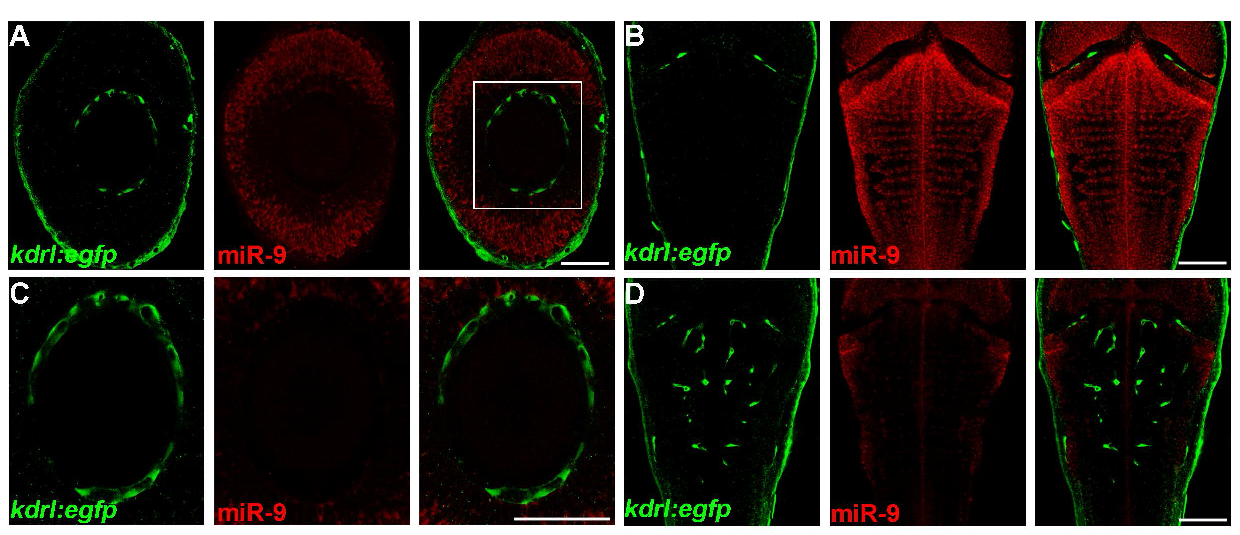
\epsfig{file=figures/zfishSnpsFigureS2.pdf,width=0.8
\linewidth,clip=,trim=0 0 0 0} \\
\end{tabular}
\caption[\emph{miR-9} expression is not detected in endothelial cells or blood vessels]{
{\bf \emph{miR-9} expression is not detected in endothelial cells or blood vessels.}
{\bf (A-D)} Confocal sections of double \emph{in
situ}/immunolabelling in \emph{Tg(kdrl:egfp)} embryos at 48 hpf showing
the absence of co-localization in the expression of the endogenous
\emph{miR-9} and EGFP protein in the retina and the hindbrain. Blood
vessels or endothelial cells are not localized in domains expressing
\emph{miR-9} in the retina {\bf (A)} and hindbrain {\bf (B)}. \emph{miR-9}
expression in not detected in \emph{kdrl:egfp+} cells in the retina {\bf (C)}
and hindbrain {\bf (D)}. Dorsal view of the brain with anterior up. Lateral
view of the retina. Scale bars: 100 $\mu$m.
}
\label{fig:zfishSnpsFigS2}
\end{figure}

\begin{landscape}
\begin{center}
\begin{longtable}{@{}>{\hspace{0pt}}p{0.1\linewidth}>{\hspace{0pt}}p{0.1\linewidth}>{\hspace{0pt}}p{0.2\linewidth}>{\hspace{0pt}}p{0.2\linewidth}>{\hspace{0pt}}p{0.06\linewidth}>{\hspace{0pt}}p{0.06\linewidth}>{\hspace{0pt}}p{0.2\linewidth}@{}}
\caption[Deeply conserved GWAS SNP screen results]{{\bf Deeply conserved GWAS SNP screen results.}
Sequence conservation blocks and gene synteny of GWAS
SNPs conserved between human and zebrafish.
}
\label{tab:zfishSnpsTabS1} \\

\hline \textbf{Variant rsIDs} & \textbf{Trait or disease} & \textbf{Human
coordinates} & \textbf{Zebrafish coordinates} & \textbf{nhmmer e-value}
& \textbf{nhmmer bit score} & \textbf{Syntenic genes (distance to
nearest transcript TSS)} \\ \hline 
\endfirsthead

\hline \textbf{Variant rsIDs} & \textbf{Trait or disease} & \textbf{Human
coordinates} & \textbf{Zebrafish coordinates} & \textbf{nhmmer e-value}
& \textbf{nhmmer bit score} & \textbf{Syntenic genes (distance to
nearest transcript TSS)} \\ \hline 
\endhead

\hline
\endlastfoot

rs6774494 & Nasopharyngeal carcinoma & hg19 chr3:169082534-169082733(+)
& danRer7 chr15:34810310-34810561(+) & 2.1E-39 & 142.6 &
MECOM(-95607): mecom(-136097)\tabularnewline
rs11190870 & Scoliosis & hg19 chr10:102979145-102979305(+) &
danRer7 chr13:28525660-28525820(+) & 2E-33 & 124.1 &
LBX1(+10326): lbx1a(+6000), TLX1(+85154): tlx1(-29839),
FBXW4(+393685): fbxw4(-210725)\tabularnewline
rs4759042 & Migraine & hg19 chr12:57377273-57377444(+) &
danRer7 chr9:49734712-49734883(+) & 3.3E-33 & 124.1 &
RDH16(-24200): dhrs9(+48910), SDR9C7(-49169): dhrs9(+48910),
HSD17B6(+197645): dhrs9(+48910)\tabularnewline
rs2307121 & Corneal structure & hg19 chr5:64625414-64625612(+) &
danRer7 chr10:11654536-11654735(+) & 1.3E-02 & 112.3 &
ADAMTS6(-66749): adamts6(+73188), PPWD1(-233550): ppwd1(-79052),
TRIM23(+281188): trim23(+151614),
CWC27(+445530): cwc27(+290628)\tabularnewline
rs17421627 & Retinal vascular caliber & hg19 chr5:87847488-87847679(+) &
danRer7 chr5:49928050-49928256(+) & 3.4E-25 & 97.8 &
MIR-9-5(+60011): mir-9-5(+24822), MEF2C(+177753): mef2cb(+114783),
TMEM161B(-282290): tmem161b(-74583)\tabularnewline
rs4880487 & Migraine & hg19 chr10:1246802-1246972(+) &
danRer7 chr24:3632273-3632449(+) & 8.6E-21 & 83.6 &
ADARB2(-562): adarb2(+228617), WDR37(+77140): wdr37(+69279),
IDI1(-151777): idi1(-77538), IDI2(-175088): idi1(-77538)\tabularnewline
rs16932455 & Capecitabine sensitivity & hg19 chr11:16040076-16040273(+)
& danRer7 chr7:28559360-28559558(-) & 1.1E-18 & 77.4 &
SOX6(-3301): sox6(-11158)\tabularnewline
rs13382811 & Myopia (severe) & hg19 chr2:145223523-145223713(+) &
danRer7 chr6:1000361-1000506(+) & 5.7E-18 & 74.6 &
ZEB2(-35481): zeb2b(-43451)\tabularnewline
rs17178006 & Hippocampal volume & hg19 chr12:65718213-65718383(+) &
danRer7 chr4:11967906-11968083(-) & 6.8E-18 & 73.7 &
MSRB3(-2357): msrb3(+5901), LEMD3(+78968): lemd3(+26539),
WIF1(-202952): wif1(-28293), HMGA2(-499613): hmga2(-41383)\tabularnewline
rs6588480 & Response to statin therapy & hg19 chr1:53978072-53978217(+)
& danRer7 chr8:18692520-18692665(-) & 5.4E-16 & 67.7 &
GLIS1(+221733): glis1b(+71584)\tabularnewline
rs12593813 & Restless legs syndrome & hg19 chr15:68036768-68036950(+) &
danRer7 chr18:19721646-19721823(+) & 9.6E-14 & 60.9 &
SKOR1(-75183): skor1b(-33588), C15orf61(+222736): C18H15orf61(+58092),
IQCH(+254506): iqch(+98454), PIAS1(-309658): pias1b(-49392),
AAGAB(-489326): aagab(-121211)\tabularnewline
rs12431307 & Obesity-related traits & hg19 chr13:80644586-80644716(+) &
danRer7 chr1:4209100-4209234(-) & 4.6E-12 & 55.2 &
SPRY2(+269143): spry2(+38248)\tabularnewline
rs4333130 & Ankylosing spondylitis & hg19 chr4:80949732-80949918(+) &
danRer7 chr5:41045298-41045471(+) & 1.2E-11 & 54.2 &
ANTXR2(+42949): antxr2a(+34553), PRDM8(-155208): prdm8b(-64707),
FGF5(-237928): fgf5(-97766),
C4orf22(-307049): C5H4orf22(-123872)\tabularnewline
rs2272046 & Polycystic ovary syndrome & hg19 chr12:66224444-66224542(+)
& danRer7 chr4:11918185-11918283(-) & 4.4E-11 & 51.5 &
HMGA2(+2712): hmga2(+8271), TMBIM4(+308224): tmbim4(+121765),
IRAK3(-358166): irak3(-62739), HELB(-471832): helb(-72528),
MSRB3(+486579): msrb3(+55661)\tabularnewline
rs2842643 & Attention deficit hyperactivity disorder &
hg19 chr6:41650647-41650827(+) & danRer7 chr11:23106736-23106903(+) &
8.8E-06 & 35.2 & TFEB(+5201): tfeb(+38515), MDFI(+36745): MDFI(+162564),
FOXP4(+112825): foxp4(+310951)\tabularnewline
rs2153271 & Freckling & hg19 chr9:16864430-16864610(+) &
danRer7 chr1:25994830-25994996(-) & 1.0E-04 & 30.9 &
BNC2(+6184): bnc2(+4776), CNTLN(-270460): cntln(-13956)\tabularnewline
rs7349332 & Hair morphology & hg19 chr2:219756333-219756404(+) &
danRer7 chr9:11675370-11675444(+) & 1.6E-03 & 26.7 &
WNT10A(-1575): wnt10a(+19316), WNT6(+31680): wnt6b(+105345),
CDK5R2(-68009): cdk5r2b(-132850), FEV(+92829): fev(+151222),
CRYBA2(+99561): cryba2b(+160934),
MIR375(+110063): dre-mir-375-2(+172880)\tabularnewline
rs7246657 & Coronary artery calcification &
hg19 chr19:37747060-37747144(+) & danRer7 chr3:8862134-8862229(+) &
1.6E-02 & 24.1 & ZNF850(483332): zgc:174234(234552)\tabularnewline
rs13414205 & Immune reponse to smallpox (secreted TNF-alpha) &
hg19 chr2:44662376-44662487(+) & danRer7 chr13:10168027-10168141(-) &
2.6E-02 & 23.7 & CAMKMT(+62544): CAMKMT(1of2)(+17764),
CAMKMT(+62544): camkmt(-171412), PREPL(-73430): prepl(-18369),
SLC3A1(+131486): slc3a1(+69409), PPM1B(+217470): ppm1ba(+124662),
LRPPRC(-439287): lrpprc(-196554)\tabularnewline
rs13095226 & Age-related macular degeneration &
hg19 chr3:99396188-99396298(+) & danRer7 chr22:29659198-29659297(-) &
1.2E-01 & 21.6 & COL8A1(-29672): col8a1b(-267444)\tabularnewline
rs1568679 & Response to antipsychotic treatment &
hg19 chr15:37349784-37349819(+) & danRer7 chr17:53456843-53456878(-) &
1.2E-01 & 21.3 & MEIS2(+36429): MEIS2(3of3)(+109701),
MEIS2(+36429): meis2a(+23451),
C15orf41(+301655): C17H15orf41(+16903)\tabularnewline
rs564148 & Response to amphetamines & hg19 chr1:34173731-34173831(+) &
danRer7 chr23:22192192-22192293(+) & 3.2E-01 & 20.1 &
PHC2(277077): phc2a(165332)\tabularnewline

\end{longtable}
\end{center}
\end{landscape}
